\epigraph{``And behold! When the numbers had been created for infinitely many days, the universe itself appeared. And the evening and the morning were the $\aleph^[\footnotemark^]$ day. And Conway looked over the rules he had made for numbers, and saw that they were very, very good. And he commanded them to be for signs, and series, and quotients, and root. Then there sprang up an infinite number less than infinity. And infinities of days brought forth multiple orders of infinities"}{Donald Ervin Knuth, Surreal Numbers \footnotemark}

\footnotetext{In order to match the the cardinal number notation, it would be more precise to write $\aleph_0$. The text will use the book notation $\aleph$.}

\footnotetext{Excerpt of the book \textit{Surreal Numbers: how two ex-students turned on to pure mathematics and found total happiness} that precedes the moment the couple define a rule for addition of numbers.}


Conway, by counting the number of spare moves a player has in combinatorial games, unveiled a new way to discover numbers. It is clear at this point that although numbers are not enough to represent games, they are the building blocks of all games, including the non-numbers. Until this point, the text showed some instances of the zero and hinted at $1$ and $-1$, and the reader may also guess on how to build any integer in RB-Hackenbush and Domineering. This chapter shows that knowing that is no more than scratching the surface of surreal numbers.

For the first parts of this section a number \gam{x_1, x_2,\, $\ldots$}{y_1, y_2,\,$\ldots$} might be called like a real number: $2, 5, 100000, \frac{1}{3}, \sqrt{10}, \pi$, but there is no reason believe this equality yet. There is also no reason to believe that $1 < 3$ or that $1 + 1 = 2$ yet. Up until this point, numbers are labels to games that trivially translated the number of spare moves a player has. However, first a few more numbers will be labeled and only then the operations and comparisons are defined.


\subsection*{Numbers Generated in Finite Steps}

It is known that \Gm{} =
\begin{tikzpicture}
	\draw[] (0.3,-0.3) rectangle ++(0.3,0.3);
	\draw[] (0,-0.3) rectangle ++(0.3,0.3);
\end{tikzpicture} = \gam{}{\gam{}{}} = \gam{}{0} and \Gm{} was labeled $-1$.
What would be a good label for \Hm = 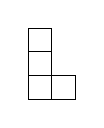
\begin{tikzpicture}
\draw[] (0.3,-0.3) rectangle ++(0.3,0.3);
\draw[] (0,-0.3) rectangle ++(0.3,0.3);
\draw[] (0,0) rectangle ++(0.3,0.3);
\draw[] (0,0.3) rectangle ++(0.3,0.3);
\end{tikzpicture}, given that it must be meaningful like described previously?\\ If it were to be labeled by a real number, which one should it be?

It is possible to find out a candidate by calculating \Gm{ + \Hm + \Hm}. To do that, one would usually find the game tree of 
\Gm{ + \Hm + \Hm} = 
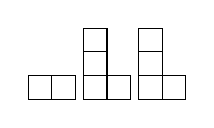
\begin{tikzpicture}
	\draw[] (-0.4,-0.3) rectangle ++(0.3,0.3);
	\draw[] (-0.7,-0.3) rectangle ++(0.3,0.3);
	\draw[] (0.3,-0.3) rectangle ++(0.3,0.3);
	\draw[] (0,-0.3) rectangle ++(0.3,0.3);
	\draw[] (0,0) rectangle ++(0.3,0.3);
	\draw[] (0,0.3) rectangle ++(0.3,0.3);
	\draw[] (1,-0.3) rectangle ++(0.3,0.3);
	\draw[] (0.7,-0.3) rectangle ++(0.3,0.3);
	\draw[] (0.7,0) rectangle ++(0.3,0.3);
	\draw[] (0.7,0.3) rectangle ++(0.3,0.3);
\end{tikzpicture}, and fill the known values bottom-up. However, it is simpler in this case. \Gm{ + 2\Hm = 0}, because whoever starts loses. Because \Gm{= -1}, a good label for \Hm is~$\frac{1}{2}$. Therefore:

$$H = \gam{{-}1, 0}{1} = \gam{0}{1} = \frac{1}{2}$$

 The second equality is true because Left would not move to $-1$ since it is a strictly worse move than moving the game to $0$. It might not seem natural for a player to be half a move up in a game, if he/she always plays one move at a time, but if it is desired that $\frac{1}{2} + \frac{1}{2} = 1$, that label makes sense for addition. It might be valuable to reiterate that \Hm is definitely positive because left wins no matter who starts, but $H < 1$, as Left does not have any spare moves, because $\Hm + \Gm = \Hm - 1 < 0$.

As one gets used to this kind of reasoning, it becomes clear that analyzing the game \gam{1}{} is the same as analyzing the game 
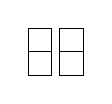
\begin{tikzpicture}
	\draw[] (0.3,-0.3) rectangle ++(0.3,0.3);
	\draw[] (0.3,0) rectangle ++(0.3,0.3);
	\draw[] (-0.1,0) rectangle ++(0.3,0.3);
	\draw[] (-0.1,-0.3) rectangle ++(0.3,0.3);
\end{tikzpicture}, but the former is not reliant on a specific ruleset. Rather, any combinatorial game has an instance equal to \gam{1}{}. However, the rules used to calculate the value of \Gm{=\gam{X}{Y}}, which are presented in the remaining of this section, help understand it better. The first practical rule in this text is finding the value of \gam{n}{} and \gam{}{{-}n}, for any natural number $n$.

Since 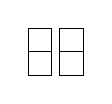
\begin{tikzpicture}
	\draw[] (0.3,-0.3) rectangle ++(0.3,0.3);
	\draw[] (0.3,0) rectangle ++(0.3,0.3);
	\draw[] (-0.1,0) rectangle ++(0.3,0.3);
	\draw[] (-0.1,-0.3) rectangle ++(0.3,0.3);
\end{tikzpicture} $= \gam{1}{}$, is it correct to assume that
$\underbrace{
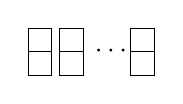
\begin{tikzpicture}
	\draw[] (1.2,-0.3) rectangle ++(0.3,0.3);
	\draw[] (1.2,0) rectangle ++(0.3,0.3);
	\draw[] (-0.1,0) rectangle ++(0.3,0.3);
	\draw[] (-0.1,-0.3) rectangle ++(0.3,0.3);
	\draw[] (0.3,0) rectangle ++(0.3,0.3);
	\draw[] (0.3,-0.3) rectangle ++(0.3,0.3);
	\node at (0.95, 0) {$\cdots$};
\end{tikzpicture}}_{n+1} = \gam{n}{}$? Yes, it is correct and the recursive nature of combinatorial games tell why. A $2\times 1$ board is equal to $1$ since Left has a move to spare. Therefore, two $2\times 1$ boards is equal to~$2$ since Left has a move to spare before reaching $1$. It is simple enough to visualize it in domineering boards. The fact is it should be simple to vizualise it in any combinatorial game. For any integer $k$, the game \gam{k}{} has the same value of the sum $\gam{k-1}{}+1$ if Left's best option $k$ is positive. If Left's best option is zero, then the game is equal to $1$, as already shown. If Left's best option is negative the result is zero, because Right cannot play, and  Left's move would result in the game $k$, which is negative, showing that whoever starts loses.  

In the case $k$ is positive, the addition $\gam{k-1}{} + 1$ was used. The notation is not the one used before, but it is possible replace $1$ with \gam{0}{}, as seen before. $\gam{k-1}{} + \gam{0}{}$ is an instance of addition described in the previous chapter. 

\begin{align*}
	\gam{k-1}{} + \gam{0}{} &\overset{def}{=} \gam{\gam{k-2}{} + \gam{0}{}, \gam{k-1}{} + \gam{}{}}{}\\
	&= \gam{\gam{k-2}{} + \gam{0}{}, \gam{k-1}{}}{}\\
	&\overset{def}{=} \gam{\gam{\gam{k-3}{} + \gam{0}{}}{}, \gam{\gam{k-2}{} + \gam{}{}}{}, \gam{\gam{k-2}{}}{}}{}\\
	&=\gam{\gam{\gam{k-3}{} + \gam{0}{}}{}, \gam{\gam{k-2}{}}{}, \gam{\gam{k-2}{}}{}}{}\\
	&=\gam{\gam{\gam{k-3}{} + \gam{0}{}}{}, \gam{\gam{k-2}{}}{}}{}\\
	&\overset{def}{\ldots}\\
	&=\underbrace{\{\{\ldots\{\{}_{k+1}\underbrace{\,|\,\}\,|\,\}\ldots\}\,|\,\}}_{k+1}\\
	&=\underbrace{\{\{\ldots\{\{}_{k} 0 \underbrace{\,|\,\}\,|\,\}\ldots\}\,|\,\}}_{k}\\
	&=\gam{k}{} = k + 1
\end{align*}

Every point discussed for \gam{X}{} is valid for \gam{}{Y}, through a similar argument. Up to this point, the integers and $\pm \frac{1}{2}$ are defined. The remaining numbers fall into three categories: the dyadic rationals - numbers of the form $\frac{a}{2^k}$, the numbers created in exactly infinite, $\aleph$, amount of steps, and the ones generated after more than infinite amount of steps. Of course the integers and $\frac{1}{2}$ fall into the first category.

In the case of $\Gm{} = \frac{1}{2} = \gam{0}{1}$, it is true that $G^L < G < G^R$. Is that always true? That is restricted for numbers, since in non-numbers \Gm{^R > G^L}. If Left makes a move from $G$ to $G^L$, is it true that Left has fewer spare moves in $G^L$ than in $G$? Before, as a side note, it was said that all possible RB-Hackenbush games are numbers, and the reason may help explain that it is true.

Suppose a game \Gm{ = \gam{X}{Y}} in which for all $x$ in $X$, $x$  is a number and for all $y$ in $Y$, $y$ is a number. Assume that $x_0$ in $X$ and $y_0$ in $Y$ are best moves for Left and Right respectively. If \Gm{} is not a number, than $x_0 \ge y_0$. Now consider \Hm an instance of RB-Hackenbush. A move in \Hm corresponds to removing a colored edge from a tree and all the edges that become disconnected to the floor. Assume again for \Hm that $x_0$ and $y_0$ are edges correspondent to the best moves for Left and Right respectively. That means that $x_0$ is similar to  
\begin{tikzpicture}
	\draw[blue, very thick] (0,0) -- (0,0.5);
	\node at (0, 0.9) {$\vdots$};
	\node at (-0.3, 0.9) {$\ddots$};
	\node at (0.3, 0.9) {\reflectbox{$\ddots$}};
\end{tikzpicture} and $y_0$ is similar to 
\begin{tikzpicture}
	\draw[red, dash pattern=on 3pt off 0.8pt, very thick] (0,0) -- (0,0.5);
	\node at (0, 0.9) {$\vdots$};
	\node at (-0.3, 0.9) {$\ddots$};
	\node at (0.3, 0.9) {\reflectbox{$\ddots$}};
\end{tikzpicture}. Is it possible that $G^{x_i} \ge G^{y_j}$?

Consider the game built by connecting $x_0$ to the floor. The game is definitely positive, as Left wins no matter who starts. If Right starts, he/she may have an available move in a edge above the one connected to the floor. Whether it is Left playing second or first, he/she may simply remove the blue edge connected to the floor, then Right has no moves remaining and loses the game. An analogous argument shows that $y_0$ in negative. Since $x_0$ is positive, the game $\Hm^{x_0}$ resulting from removing this positive branch is less positive, or more negative, than \Hm. The same way, $\Hm^{y_0}$ is more positive or less negative that \Hm. This fact, in turn, means that \Hm is a number.

Other phrasing for ``all RB-Hackenbush games are numbers" is ``it is not possible to make a move that improves your position in  RB-Hackenbush", or, ``Left cannot make a movement that increases the value of \Gm{}". Visualizing it brings the general idea why, in numbers, $G^L < G < G^R$. A more general approach is to consider, by induction, that $\Gm{^{LL}} < \Gm{^L} < \Gm{^{LR}}$ and $\Gm{^{RL}} < \Gm{^R} < \Gm{^{RR}}$. \Gm{^{LL}} translates to any possible Left move in \Gm{^L} and the others are defined similarly.

Consider the sum $\Gm{} - \Gm{^L}$. Before proceeding, the subtraction in this field means adding the negation. The negation of \gam{X}{Y} is \gam{-Y}{-X}. A good way to think of negation of a game \Gm{} as the same game \Gm{}, but with roles reversed. In the case of RB-Hackenbush for example, in ${-}\Gm{^L}$, Left plays the red edges. If Left starts, he/she can move to $\Gm{^L} - \Gm{^L} = 0$ and win the game. If Right starts, the game may be move to $\Gm{^R} - \Gm{^L}$ or $\Gm{} - \Gm{^{LR}}$. In the first case, it is clear that $\Gm{^R} - \Gm{^L} > 0$ because, from the definition of numbers, \Gm{^R} $>$ \Gm{^L}.
In the second case Left can move to $\Gm{^L} - \Gm{^{LR}}$, which is positive due to the induction hypothesis. Therefore, regardless who starts in $\Gm{} - \Gm{^L}$, Left wins, so the game is positive, meaning \Gm{>\Gm{^L}}. A similar argument shows that \Gm{<\Gm{^R}}.

Knowing this, however, is not enough to find the value of G. If $G = \{3 | 10\}$, it is clear that $3 < G < 10$ but what is the value of G? The simpler number that fits this interval, 4. What is called simpler is the minimal-birthday number that fits the interval. The word birthday comes from the initial analogy used to describe the creation of all the numbers. Before visiting the birthday tree and finishing explaining the simplicity principle, it is necessary to visit the definition of the comparison $\leq$.

Just like the definition of addition, the comparison is also done using game trees so it is the same for numbers and non-numbers. Consider the games \Gm{} and \Hm. \Gm{\leq \Hm} if they are equal or \Hm is more positive than \Gm{}. This condition is met if $\Hm > G^L$ and \Gm{<H^R}. These restrictions enforce that \Gm{=\gam{G^L}{G^R, H^R}} and $\Hm = \gam{G^L,H^L}{H^R}$, which guarantee the desired relation.

The birthday tree is the name given to the hierarchical structure that contains the definition of all surreal numbers. The tree is composed of layers, called generations, and each layer is a set of all the numbers formable with the available symbols. The zeroth generation is simply the set $\{0\} = \{\gam{}{}\}$. The first generation is the set $\{{-}1,0,1\}=$ \{\gam{}{0}, \gam{}{}, \gam{0}{}\}. The second is $\{-2,-1,\frac{-1}{2},0,\frac{1}{2},1,2\}$ and is equal to $\{\gam{}{{-}1},\gam{}{0},\gam{{-}1}{0},\gam{}{},\gam{0}{1}\gam{0}{},\gam{1}{}\}$. $0$ is called a zeroth generation number and $1$ and ${-}1$ are first generation numbers.

An important aspect of the generations is that, although labeling is not defined yet, they are fully ordered. Ordering is necessary for the simplicity rule because, as said before, \Gm{^L < \Gm{} < \Gm{^R}}. In order to find the value of \Gm{}, it is necessary to find a generation that contains both \Gm{^L} and \Gm{^R}, order it using the previously defined $\leq$ operation and find the oldest number lying strictly between \Gm{^L} and \Gm{^R}.

It is possible, however, to find cases where there are no numbers between \Gm{^L} and \Gm{^R}. In these case, one could look for a fitting number in the next generation. Another way to solve this is to notice that this cases occur if and only if both options are from the same generations and are neighbors in that generation. This condition implies that \Gm{^L = \frac{p}{2^q}} and \Gm{^R = \frac{p+1}{2^q}}. In this cases, the number in the next generation that lies strictly between them is the number \Gm{} and this number is labeled $\frac{2p + 1}{2^{q+1}}$.

The rules and definitions up until this point add up to:

\begin{center}
\Gm{ =} 
$
\begin{cases}
	0, &\text{if } G^L < 0 < G^R\\
	n+1, &\text{if } \Gm{= \gam{n}{}}\\
	-n-1, &\text{if } \Gm{= \gam{}{{-}n}}\\
	\frac{2p + 1}{2^{q+1}}, &\text{if } \Gm{= \gam{\frac{p}{2^q}}{ \frac{p+1}{2^q}}}\\
	\text{search the tree} &\text{otherwise}
\end{cases}
$
\end{center}

\vspace{0.6em}Some examples are $\frac{1}{4} =$ \gam{\frac{1}{10}}{\frac{3}{10}}, $\frac{1}{8} =$ \gam{0}{\frac{1}{4}}, $10 =$ \gam{9}{}, $1 =$ \gam{\frac{1}{2}}{}. The first and last examples require some manipulation as they would require a search on the birthday tree, as described previously. This would be a problem because both options of the first example would require an infinite number of generations to be created. However, since the embedded real numbers ought to be ordered the same and since surreals numbers are generated successively, the first number that fits the interval is the simplest that fits. Since $\frac{1}{10} < \frac{1}{4} < \frac{3}{10}$ and no older number older fits, the equality stands.

The remaining problematic example is $1 =$ \gam{\frac{1}{2}}{}. Consider the games, which happen to be numbers, \Gm{= \gam{0}{}} and $H = \gam{\frac{1}{2}}{}$. $G = 1$, directly from the simplicity rules. It is said that $H = 1$, but that is not a direct implication. It is possible, however, to show $G \leq H \leq G$. $H \leq G$, because $0.5$ is the only Left option of $H$, there are no Right options in $G$ and $0.5 < G = 1$. $G \leq H$, because $0$ is the only Left option of $G$, there are no Right options in $H$ and $0 < H$. The last inequality, $0 < H$, is true because in the game $H$, Left wins no matter who starts, and this means the game is positive.

It is possible to think of many other cases that require other manipulations to fall into the precisely defined rules. The reality is that the first four rules and the $\leq$ comparison are enough to label all the numbers. The fuzzy notion of simplicity brought in the last few paragraphs helps finding and understanding the reason for labels given but it is not necessary. The `Simplicity Rules' are actually just the first four rules.

\begin{center}
	\Gm{ =} 
	$
	\begin{cases}
		0, &\text{if } G^L < 0 < G^R\\
		n+1, &\text{if } \Gm{= \gam{n}{}}\\
		-n-1, &\text{if } \Gm{= \gam{}{{-}n}}\\
		\frac{2p + 1}{2^{q+1}}, &\text{if } \Gm{= \gam{\frac{p}{2^q}}{ \frac{p+1}{2^q}}}
	\end{cases}
	$
\end{center}

\subsection*{Numbers generated after infinite steps}

The formula above only allows \Gm{} to have an infinite amount of values, but the dimension of this infinity might not approach the stated in the beginning of the section yet. The remaining numbers are hidden in the end of infinite games. Infinite games, in this section, indicate board sizes that infinite, not infinite play, because, as explained before, this text only deals with short games. 

\begin{figure} [!ht]
\begin{center}
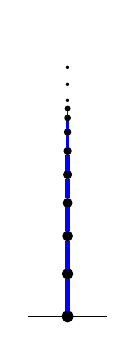
\begin{tikzpicture}
	\begin{scope} [every node/.style={scale=0.3, style=circle, draw, fill=black}]
		\node [scale=1.4] (1) at (0, -1.80){};
		\node [scale=1.3] (2) at (0, -1.26){};
		\node [scale=1.2] (3) at (0, -0.78){};
		\node [scale=1.1] (4) at (0, -0.36){};
		\node [scale=1]   (5) at (0, 0)      {};
		\node [scale=0.9] (6) at (0, 0.3)  {};
		\node [scale=0.8] (7) at (0, 0.54) {};
		\node [scale=0.7] (8) at (0, 0.72) {};
		\node [scale=0.6] (9) at (0, 0.84) {};
		\node [scale=0.2, fill=white, draw=none] at (0, 1.1) {$\vdots$};
	\end{scope}
	\draw (-0.5,-1.80) -- (0.5, -1.80);
	\draw[blue, ultra thick] (1)--(2);
	\draw[blue, ultra thick] (2)--(3);
	\draw[blue, ultra thick] (3)--(4);
	\draw[blue, ultra thick] (4)--(5);
	\draw[blue, ultra thick] (5)--(6);
	\draw[blue, thick] (6)--(7);
	\draw[blue, thick] (7)--(8);
	\draw[blue] (8)--(9);
	\node[scale=1.5] at (0, 1.3) {\scriptsize$\vdots$};
\end{tikzpicture}
\end{center}
\end{figure}

In the game above, Left has an infinite number of possible moves, but his/her move always leads to an integer. What is the value of this game? \gam{1,2,...}{}, the one more than the largest natural number. This number has been baptized much earlier in mathematics. It was called $\omega$, the first ordinal number, and the label is kept in the surreal numbers. It might not be as straight forward as finitely generated numbers, but the principle to calculate the value is the same.

For any finite number of red edges in \Gm{}, if you add the game above to \Gm{}, the result will be positive. However, it is also very simple to verify that $\omega$ is by far not the largest possible advantage. One simple  example for that is the following section.

$\omega$ is one of numbers generated in the $\aleph$ generation. Another is the number \gam{0}{\frac{1}{1}, \frac{1}{2}, \ldots}, labeled $\epsilon$. This number is positive, as Left wins no matter who starts, but it is smaller than any positive real number. A game with value $\epsilon$ may be simply the game of RB-Hackenbush starting with a blue edge and following with an infinite number of red edges.

These numbers are special in the sense that they are the first non-real numbers to show up, but they are not the only non-reals and they are not the only members of their generation. The integers and dyadic rationals show up in earlier generations, but the remaining reals all show up in the $\aleph$ generation. Chapter 5 will develop this topic a little further but, in general, it is not paramount to the topic of temperature.

\subsection*{Numbers generated after more than infinite steps}

\begin{figure} [!ht]
\begin{center}
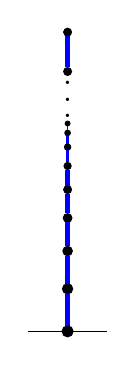
\begin{tikzpicture}
	\begin{scope} [every node/.style={scale=0.3, style=circle, draw, fill=black}]
		\node [scale=1.4] (1) at (0, -1.80){};
		\node [scale=1.3] (2) at (0, -1.26){};
		\node [scale=1.2] (3) at (0, -0.78){};
		\node [scale=1.1] (4) at (0, -0.36){};
		\node [scale=1]   (5) at (0, 0)      {};
		\node [scale=0.9] (6) at (0, 0.3)  {};
		\node [scale=0.8] (7) at (0, 0.54) {};
		\node [scale=0.7] (8) at (0, 0.72) {};
		\node [scale=0.6] (9) at (0, 0.84) {};
		\node [scale=0.2, fill=white, draw=none] at (0, 1.1) {$\vdots$};
		\node [scale=1] (10) at (0, 1.5) {};
		\node [scale=1] (11) at (0, 2) {};
	\end{scope}
	\draw (-0.5,-1.80) -- (0.5, -1.80);
	\draw[blue, ultra thick] (1)--(2);
	\draw[blue, ultra thick] (2)--(3);
	\draw[blue, ultra thick] (3)--(4);
	\draw[blue, ultra thick] (4)--(5);
	\draw[blue, ultra thick] (5)--(6);
	\draw[blue, thick] (6)--(7);
	\draw[blue, thick] (7)--(8);
	\draw[blue] (8)--(9);
	\node[scale=1.5] at (0, 1.3) {\scriptsize$\vdots$};
	\draw[blue, ultra thick] (10)--(11);
\end{tikzpicture}
\end{center}
\end{figure}

The game above is an infinite stack of blue edges with another one on the top. One could wrongly argue that this additional edge on the top is simply part of the infinite stack. This is a wrong argument because this additional edge on the top allows Left to move to $\omega$, and therefore, has the value of $\omega+1$, making the games different. The reason why in this case you can move to $\omega$ is that you can move on the top-most edge, while before, there was no top-most edge. This detail is paramount to understanding the statement found on the epigraph of this section.

A hypothetical John Horton Conway wrote the paragraph found on the epigraph near a cave close to the edge of the Indian Ocean, where a couple of future mathematicians went to find themselves. The words attributed to Conway by Knuth say that in the $\aleph$th day the universe appeared. That is because Knuth realizes that in that specific days all real numbers are generated.

However, again, accordingly to the hypothetical Conway, days kept passing by and more numbers were generated. The number $\omega+1$ is one of the infinitely many surreal numbers that are not real numbers. However, this is not the end of the story. In fact, even considering that $\omega + \omega + ...$ and $\omega^\omega$ are also generated in the same format, the important part might again be missed. That is because looking at large numbers is not the only way forward.

Now that $\epsilon$ is a known members of the $\aleph$ generation, it is possible to make numbers like \gam{0}{\epsilon} and \gam{-\epsilon}{0} and also games like \gam{1}{1 + \epsilon} and \gam{1-\epsilon}{1}. As the generations keep getting created it is easy to see that there are infinite numbers that are positive but less than any positive real number. In fact if taking the example around 1, it is possible to notice that between any two real numbers there are infinite non-real numbers. These non-real numbers are called infinitesimals.

There are still more non-real number that are not infinitesimals nor cardinals. A good example is the number $\sqrt{\omega} = \gam{1,2,3,\ldots}{\omega, \frac{\omega}{2},\frac{\omega}{4},\ldots}$. To verify that the label $\sqrt{\omega}$ is proper one would need to learn the definition of multiplication and verify that $\sqrt{\omega} \cdot \sqrt{\omega} = \omega$. As this text makes no use of multiplication this is not going to be verified. This example serves only to contribute to the point that there are truly many numbers originating from the simplicity rules.

\subsection*{The Surreal Numbers}

This text presents only few characteristics of the surreal numbers as they are not the focus. It is also not necessary to know every algebraic property of numbers to go forward with the study of temperature this text focus on. However, it so happens that with very few construction rules, the numbers contain all the reals, the ordinals, the infinitesimals numbers.

Because of its extremely simple definition and big expressiveness, it is an extremely interesting topic. The idea that the number of spare moves a player has might not be a real number might not be confusing, but it should be somewhat hard to accept. It is true that this fact is based on the construction Conway made and it is not necessarily true for all ways to analyze games, but the straight forward way of using game trees to build numbers lead to this characteristic.

Because the creation/discovery of surreals is very recent, it definitely makes people apprehensive as it is not clear if its properties are good or bad. The mathematician Phillip Ehrlich is an eloquent participant in this discussion. He makes the point that the surreals do not have an intrinsic problem and that they show an unifying nature between paths in mathematics. In one of his papers, Ehrlich proposes that, while the real numbers form, on his words, an arithmetic continuum, the surreals form the absolute arithmetic continuum\cite{7}.

However, it is still a problem converting the domain of typical studies, such as calculus, from the reals to the surreals. Integrals of functions in the surreals are particularly hard to define. In the 2015 revision of their paper \cite{8}, Salzedo and Swaminathan made important contributions. For reference, they proved the intermediate value theorem in \textbf{No}, how the class of all surreal numbers is called. However, for example, they used a definition of integration that, although solving a problem with previous definitions, they make it clear that other problems persist.

As the same authors point-out: ``The `Conway-Norton'\footnote{In ONAG 2nd edition page 228, Conway  tells that Norton's definition of integrals do not have desired properties.}
integral failed to have standard properties of real integration, however, such as translation
invariance: $\int_a^bf(x)dx = \int_{a-t}^{b-t}f(x+t)dx$, for any surreal function f and $a,b,t\in$ \textbf{No}. While Fornasiero fixed this issue \cite{9}, the new integral, like its predecessor, yields
$exp(\omega)$ instead of the desired $exp(\omega)-1$ for $\int_0^{\omega}exp(x)dx$". In the ``Open Questions" section of  the paper, the authors tell that there are still problems with their definition, meaning that the conversion of domains in integral studies is not completed, at least by 2015.

While many questions remain open, however, it is still possible to work with a subset of the surreals that only contain the reals for example. The remaining of the text does not require profound knowledge of anything that is not mentioned in regards to numbers.









